\chapter{Superconductivity and quench: an overview}
\label{chp:soupcond-quench}
In this chapter I will explain some of the very basic concepts linked to superconductors and
superconductor quench.
\section{Superconductivity in theory}
\label{sec:soupcond}
Electronic motion in metallic or insulating materials is a very well studied and documented
phenomenon. Electrons passing through any material, endure a varying amount of disturbance in their
motion based on the type and structure of the material, this disturbance is known as resistivity $\rho$.
Given a sample of a material of length $l$ and cross-section $A$ we can compute the resistivity as
shown in \Cref{eq:resistivity-cable}
\begin{equation}
	\label{eq:resistivity-cable}
	\rho = \frac{RA}{l} = \frac{m}{ne^2\tau}
\end{equation}
As highlighted in the second part of \Cref{eq:resistivity-cable}, the resistivity of a
material can be seen as a function of:
\begin{itemize}
	\item The mass of the electron $m$,
	\item The charge density $n$,
	\item The charge of the electron $e$
	\item The relaxation time of the electron, which is the time interval occurring between two
	      successive electronic collisions $\tau$.
\end{itemize}
This other formulation allows us to interpret the resistivity based on the amount of electronic
interactions registered within the sample.

\medskip

Given a sample of any material, let's suppose that its resistivity was measured at a reference
temperature $T_0$ and one is interested in the resistivity at a certain temperature $T$, it's
possible to link the resistivity at temperature $T$, $\rho_T$, to the reference resistivity,
$\rho_0$ and the temperature change $T - T_0$ multiplied by a regularization term.
\begin{equation}
	\label{eq:resistivity-func-of-temp}
	\rho_T = \rho_0[1 + \alpha(T - T_0)]
\end{equation}
$\alpha$ is known as the temperature coefficient of resistivity, which is the ratio of resistance change to temperature change.

\Cref{eq:resistivity-func-of-temp} and the second part of \Cref{eq:resistivity-cable} show two
different aspects of the same measurement, but it's clear that the amount of resistance that a
certain material imposes to the passage of electrons inside its structure is dependent on the
temperature of the sample.

\medskip

Based on their values of resistivity materials can be divided between metals and insulators. Metals
will have a very low value of resistivity (usually less than $10^{-5}$) while insulators impede the
passing of electric current.
In \cite{slimani2022superconducting} solid band theory is used in conjunction with \Cref{eq:resistivity-func-of-temp} to explain the behavior of both metals and insulators in terms of
freedom of movement of the electrons flowing through the crystalline reticle. Increasing the
operation temperature of a sample yields opposite results based on the material: if the sample is a
metal then increasing the operating temperature will provoke an increase in resistivity, if the
sample is an insulator then the resistivity will decrease and, in some cases, the insulator might
start behaving like a metal, favoring the passing of electricity \cite{slimani2022superconducting}.

\bigskip

In 1911 \cite{invention-superconductivity} it was discovered that if a sample of mercury was cooled
until it reached the temperature of $4.2K$ the resistance exerted by the sample on a current travelling
through it fell from a definite real value to $0$, as can be
seen in \Cref{img:mercury-resistance}, the mercury sample had reached the superconducting state.
\begin{figure}
	\centering
	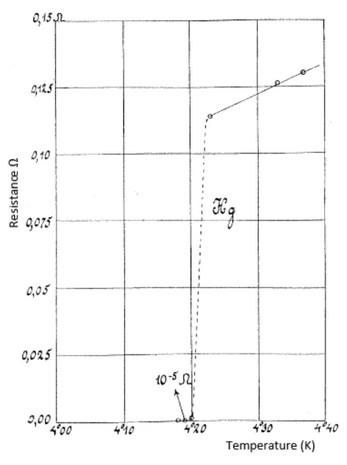
\includegraphics[width=0.5\textwidth]{./img/mercury-resistance.png}
	\caption{The resistance of Mercury in function of the temperature of the sample, taken from
		\cite{tsukerman2020compendium}}
	\label{img:mercury-resistance}
\end{figure}

Later studies discovered that many materials, pure and alloy, could be brought to the
superconducting state as long as three conditions were met:
\begin{itemize}
	\item The temperature of the sample didn't exceed the critical temperature $\tc$,
	\item The current density passing through the sample didn't exceed the critical current
	      density $\jc$,
	\item The magnetic field acting on the material didn't exceed the critical magnetic field $\bc$.
\end{itemize}

When a material reaches the superconducting state it exhibits perfect diamagnetism, which means that
the material is able to perfectly repel magnetic fields, a simple experimental proof of this effect
is given by magnetic levitation. This capacity to repel magnetic fields was first observed by
Meissner and Ochsenfeld in 1933 \cite{meissner1933}. In 1935 the London's equations proved that
superconductors, in some situations, do not exhibit a perfectly diamagnetic behavior and allow the
penetration of magnetic fields down to a certain depth, known as the London's penetration depth
\cite{london1935}. This property of superconductors was actually already theorized by Dutch
physicist Geertruida de Haas-Lorentz, who published some preliminary research in
\cite{fokker1925physica}.

The diamagnetic properties of superconductors depend on the strength of the applied magnetic field
and the material used to build the sample. Two different Types of superconductors have been
identified and studied\footnote{In general superconductor behavior can be explained through
	Ginzburg-Landau theory \cite{Cyrot1973} but very recent research has proven that not every
	superconductor can be described using the GL equation as shown in
	\cite{diamantini2023typeiiisuperconductivity}, due to how recent the research is it seems
	that nobody other than Diamantini published in the field of Type III superconductivity}, in the following I will provide a brief description of each.

\section{Type I superconductors}
\label{sec:type1}
As it can be seen in \Cref{img:type1-transition} Type I superconductors are characterized by a very
sharp fall of their magnetization, which measures the amount of induced or
permanent magnetic dipole moment of a magnet per unit volume \cite{polarization-magnetization}, once
the applied magnetic field reaches $\bc$.
\begin{figure}
	\centering
	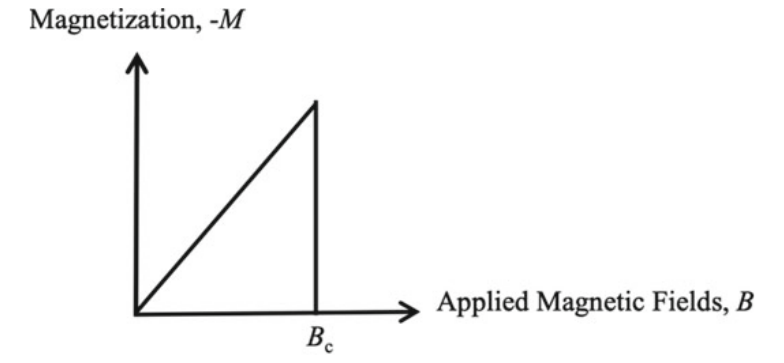
\includegraphics[width=0.75\textwidth]{./img/type1.png}
	\caption{Magnetization of a superconducting coil plotted agains the external magnetic field
		\cite{slimani2022superconducting}}
	\label{img:type1-transition}
\end{figure}
As long as the applied magnetic field is less than $\bc$, Type I superconductors exhibit perfect
diamagnetism, but once the material undergoes a transition to the normal-conducting
state (which will be referred to as \emph{quench} from now on) the magnetic dipole exerted by the
superconductor falls to zero (or a negligible value) allowing magnetic field penetration and making such materials unsuitable for the kind of environments and applications such the ones covered by this thesis.

\section{Type II superconductors}
\label{sec:type2}
Type II superconductors are usually dirtier materials compared to Type I superconductors, in most
cases the material is an alloy, this characteristical impurity gives Type II superconductors an edge
over Type I due to the magnetization degrading gracefully with the increase of applied magnetic
field. A schema similar to \Cref{img:type1-transition} can be seen in \Cref{img:type2-transition}.
\begin{figure}
	\centering
	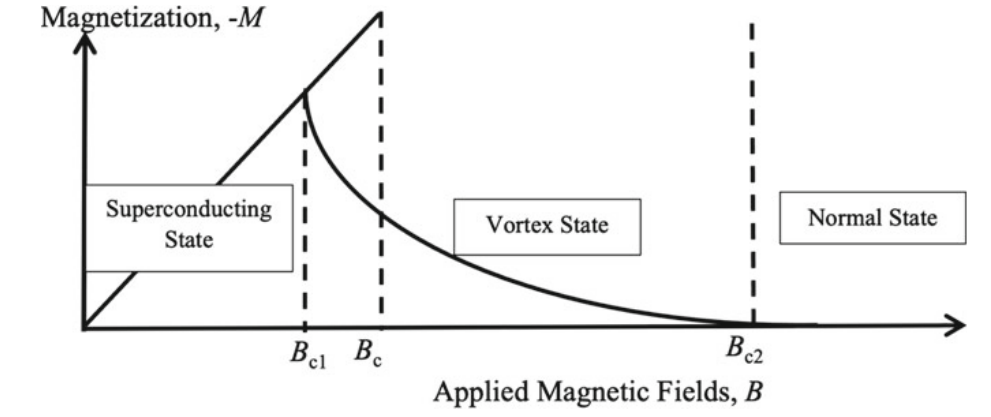
\includegraphics[width=0.75\textwidth]{./img/type2.png}
	\caption{Magnetization of a type II superconducting coil plotted against the external magnetic field
		\cite{slimani2022superconducting}}
	\label{img:type2-transition}
\end{figure}

\medskip

Type II superconductors, while the applied magnetic field is less than $B_{C1}$ have the same
diamagnetic properties of Type I superconductors but, instead of having a very sharp transition from the superconducting state to
the normal-conducting state once $B_{C1}$ is reached, these materials have an intermediate state referred to as the vortex or hybrid
state.

\medskip

In the vortex state the external magnetic field is penetrating the surface of the superconductor, but the
flux lines are constrained in particular structures pinned within the reticle of the
superconductor, called Abrikosov vortices or fluxons \cite{abrikosov-vortices}; a vortex is a supercurrent
following a ring trajectory surrounding the magnetic field lines that started penetrating the
material. Since the ring structure is extremely stable \cite{fujita-theory-HTS}, as long as the
fluxons are pinned in place, the material remains
locally superconductive, vortices are usually anchored to imperfections in the material, that is why
(as was said earlier) alloys and dirtier materials are usually Type II superconductors.

Type II superconductors are usually the kind of materials used in applications such as the one
discussed in this thesis due to the high resilience to the influence of external magnetic fields.

\section{Quench}
As was said in a previous section, whenever a superconductor performs a transition to the
normal-conducting state, therefore developing a resistance, it's undergoing a quench. This
transition might be particularly destructive if left unchecked, because the presence of resistance
in a superconductor that carries a very high current might cause it to burn. That is why, normally,
in the field of accelerator physics, superconducting magnets are accompanied with QPS (Quench
Protection Systems), which interrupt power delivery whenever one of the coils develops a voltage
that is higher than a certain threshold value.

\medskip

The work for this thesis is built around the work done by Samuele Mariotto, INFN researcher, in
\cite{mariotto2022} \cite{mariotto2022-generic}, the objective of the original papers was to find a
way to reliably and analytically solve the QLP (Quench Location Problem) through the method or
harmonic decomposition of the residual magnetic field registered in the superconductor after a
discharge.
